\chapter{Minería de Procesos}\label{sec:chapterIII}
\addcontentsline{toc}{chapter}{Minería de Procesos}

Como se ha comentado antes, cualquier posible evaluación de los alumnos basada meramente en los objetivos alcanzados es sólo una visión estática, sin muchas pistas sobre la dinámica que les ha llevado hasta ese punto. No sabemos muy bien cómo han llegado los alumnos hasta ahí y esta información es la clave para identificar a los grupos con dificultades que podrían necesitar la ayuda del profesor. Por lo tanto, vamos a emplear técnicas de Minería de Procesos \cite{aalst2016} para extraer las diferentes secuencias de eventos correlacionados del conjunto de datos original.

\section{Extracción de los procesos con DISCO}

Para la extracción de los procesos ocultos se empleará la muy conocida suite de minería de procesos Disco \cite{gunther2012disco}. Disco es una herramienta que permite crear mapas visuales a partir de los registros en cuestión de minutos.

\emph{Fuzzy Miner} \cite{gunther2007fuzzy} es un algoritmo de minería de procesos muy flexible y sólido que está detrás de Disco. En un proceso típico minado con Disco, cada actividad del proceso se etiqueta como en la Tabla \ref{tab:sequence} e incluye las frecuencias tanto de las actividades como de las transiciones entre actividades. Por lo tanto, la frecuencia de cada actividad representa el número de veces que esta actividad aparece en $B^g$. Por otro lado, la frecuencia de cada transición entre las actividades $x$ e $y$ representa el número de veces que la actividad $x$ aparece inmediatamente antes de la actividad $y$ en $B^g$.

Para crear los diagramas de Disco, se extraerán los campos de información más importantes del dataset:
\begin{enumerate}
\item El \emph{identificador del caso}, extraído de una clave aleatoria generada al principio de cada operación \texttt{LOGIN} y que distingue de manera unívoca cada sesión de trabajo de los estudiantes.
\item El \emph{agente}, que se refiere al nombre del grupo de estudiantes.
\item La \emph{fecha} y \emph{hora} a la que se registró la transacción.
\item El campo \emph{actividad} (\texttt{Activity}), que refleja la acción de los alumnos en el mundo virtual.
\item Varios campos de tipo \emph{recurso} (\texttt{Resource}) que proporcionan información adicional que puede sernos de utilidad a la hora de filtrar los registros.
\end{enumerate}

Así pues, se importarán el dataset de dos maneras diferentes, con el objetivo de estudiar tanto la frecuencia con que cada problema o mapa ha sido visitado como las acciones compuestas mapa-porcentaje superado. En la primera importación la \texttt{Activity} es el problema y el identificador del caso es el grupo. En la segunda importancia, por el contrario, la \texttt{Activity} es la composición del problema y el milestone y el identificador del caso son las sesiones. Las Figuras \ref{fig:problems} y \ref{fig:compound} muestran los diagramas obtenidos en cada uno de los casos.

\begin{figure}[H]
    \centering
    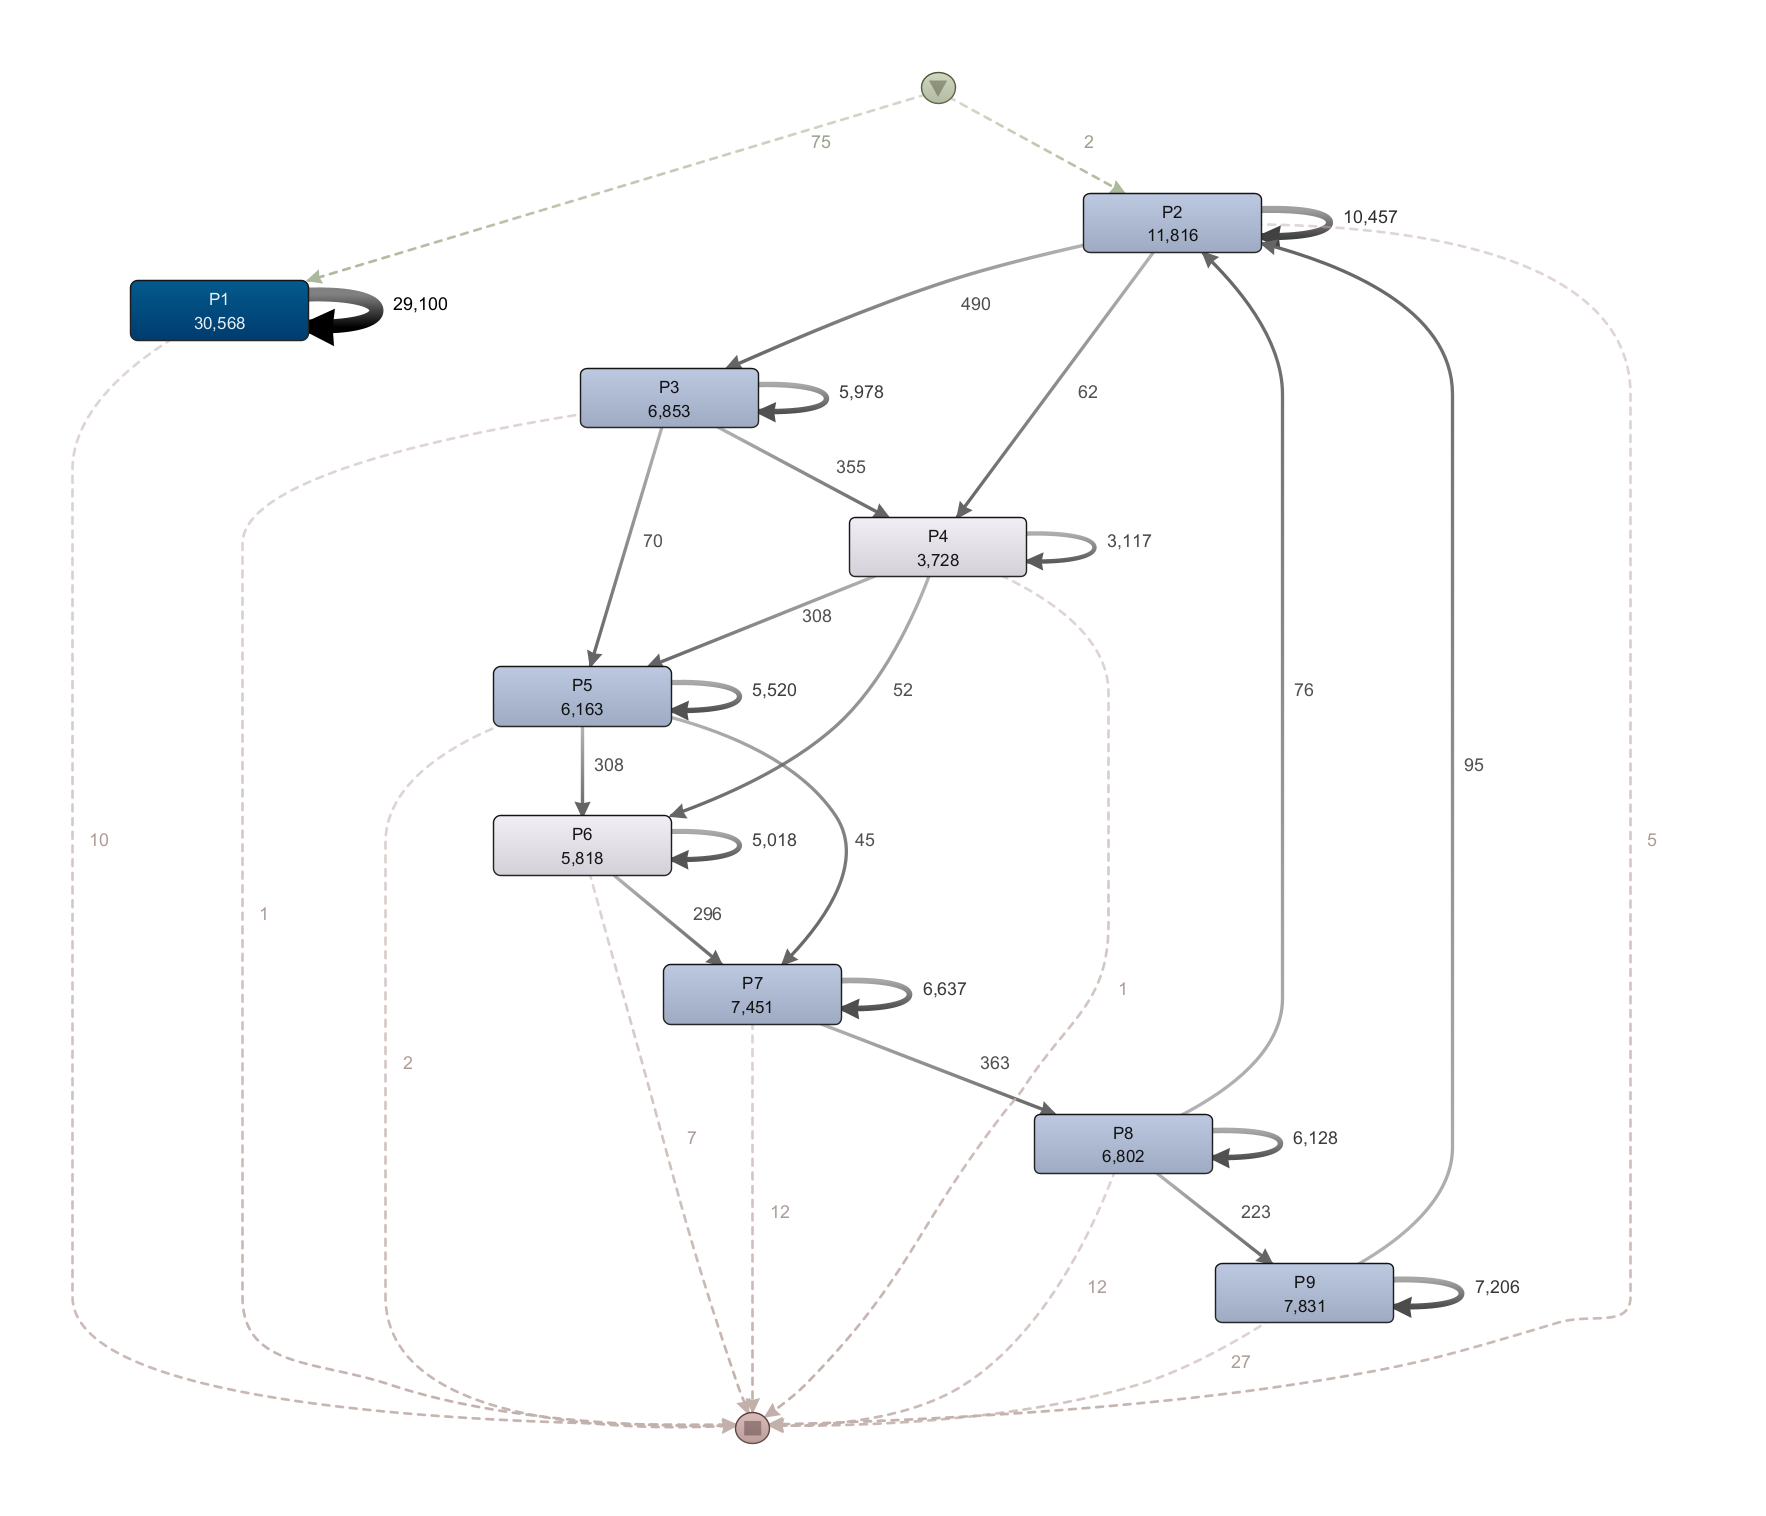
\includegraphics[width=\textwidth]{procesos/problems.png}
    \caption{Análisis de procesos del dataset (\texttt{Activity} problema y \texttt{CaseId} grupo). Contiene el $100\%$ de las actividades y el $80\%$ de los caminos.}
    \label{fig:problems}
\end{figure}

\begin{figure}[H]
    \centering
    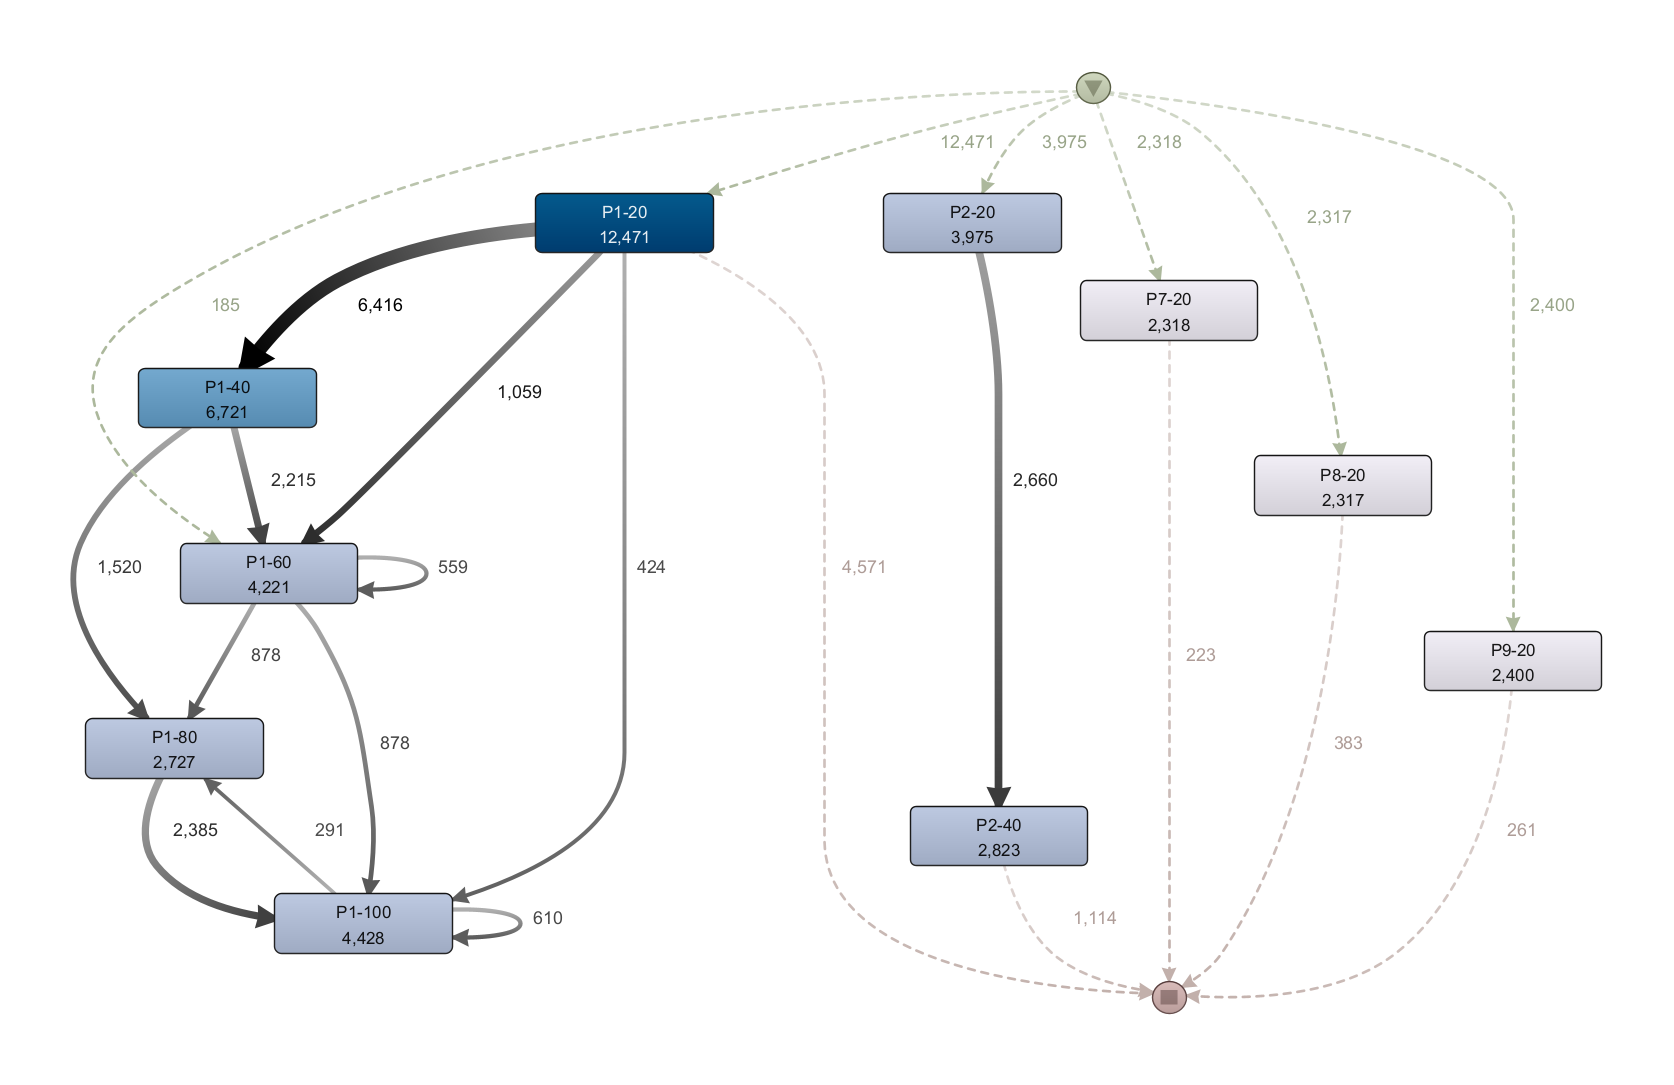
\includegraphics[width=\textwidth]{procesos/compound.png}
    \caption{Análisis de procesos del dataset (\texttt{Activity} problema-milestone y \texttt{CaseId} sesión). Contiene el $20\%$ de las actividades y el $20\%$ de los caminos.}
    \label{fig:compound}
\end{figure}

No obstante, a pesar de que tener una visión global del comportamiento de todos los grupos puede ayudar, nuestro objetivo final es poder caracterizar los comportamientos de los grupos y poder discernir, usando los datos del diagrama, si un grupo está en riesgo de obtener un rendimiento peor del esperado. Es por esto que nos será más interesante segmentar por grupos. Así pues, filtrando por el grupo \texttt{DBA 1516 P2 GA}, obtenemos los diagramas de las Figuras \ref{fig:problemsDBA1516P2GA} y \ref{fig:compoundDBA1516P2GA}.

\begin{figure}[H]
    \centering
    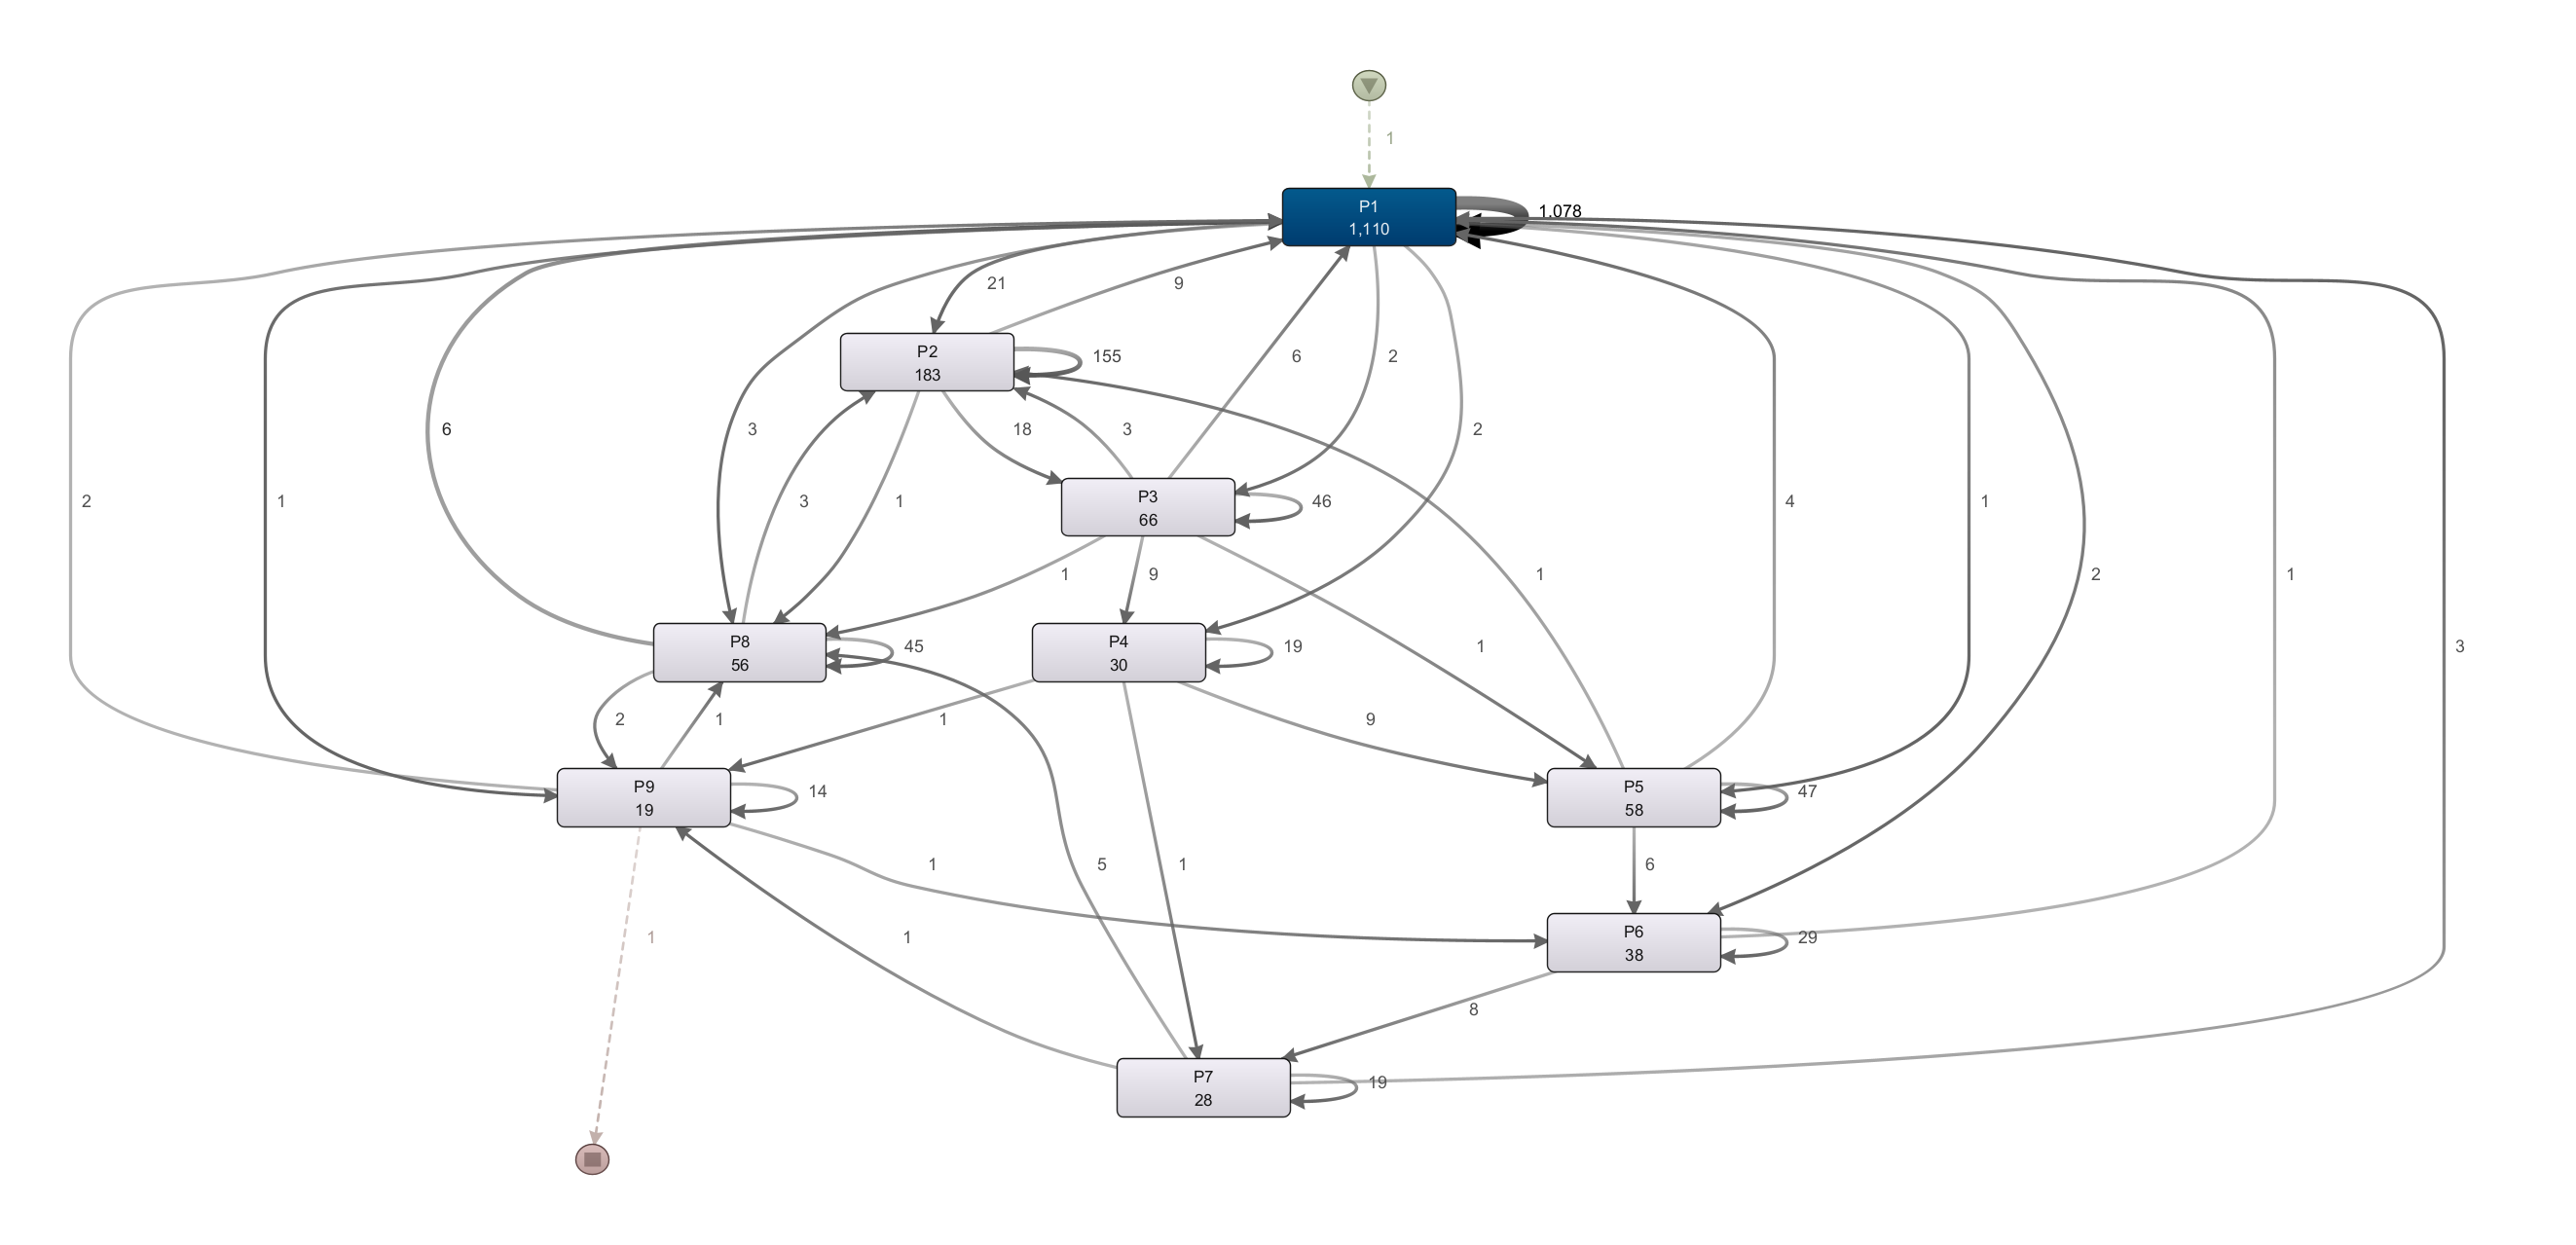
\includegraphics[width=\textwidth]{procesos/DBA1516P2GAProblems.png}
    \caption{Análisis de procesos del grupo \texttt{DBA 1516 P2 GA} (\texttt{Activity} problema y \texttt{CaseId} grupo). Contiene el $100\%$ de las actividades y el $100\%$ de los caminos.}
    \label{fig:problemsDBA1516P2GA}
\end{figure}

\begin{figure}[H]
    \centering
    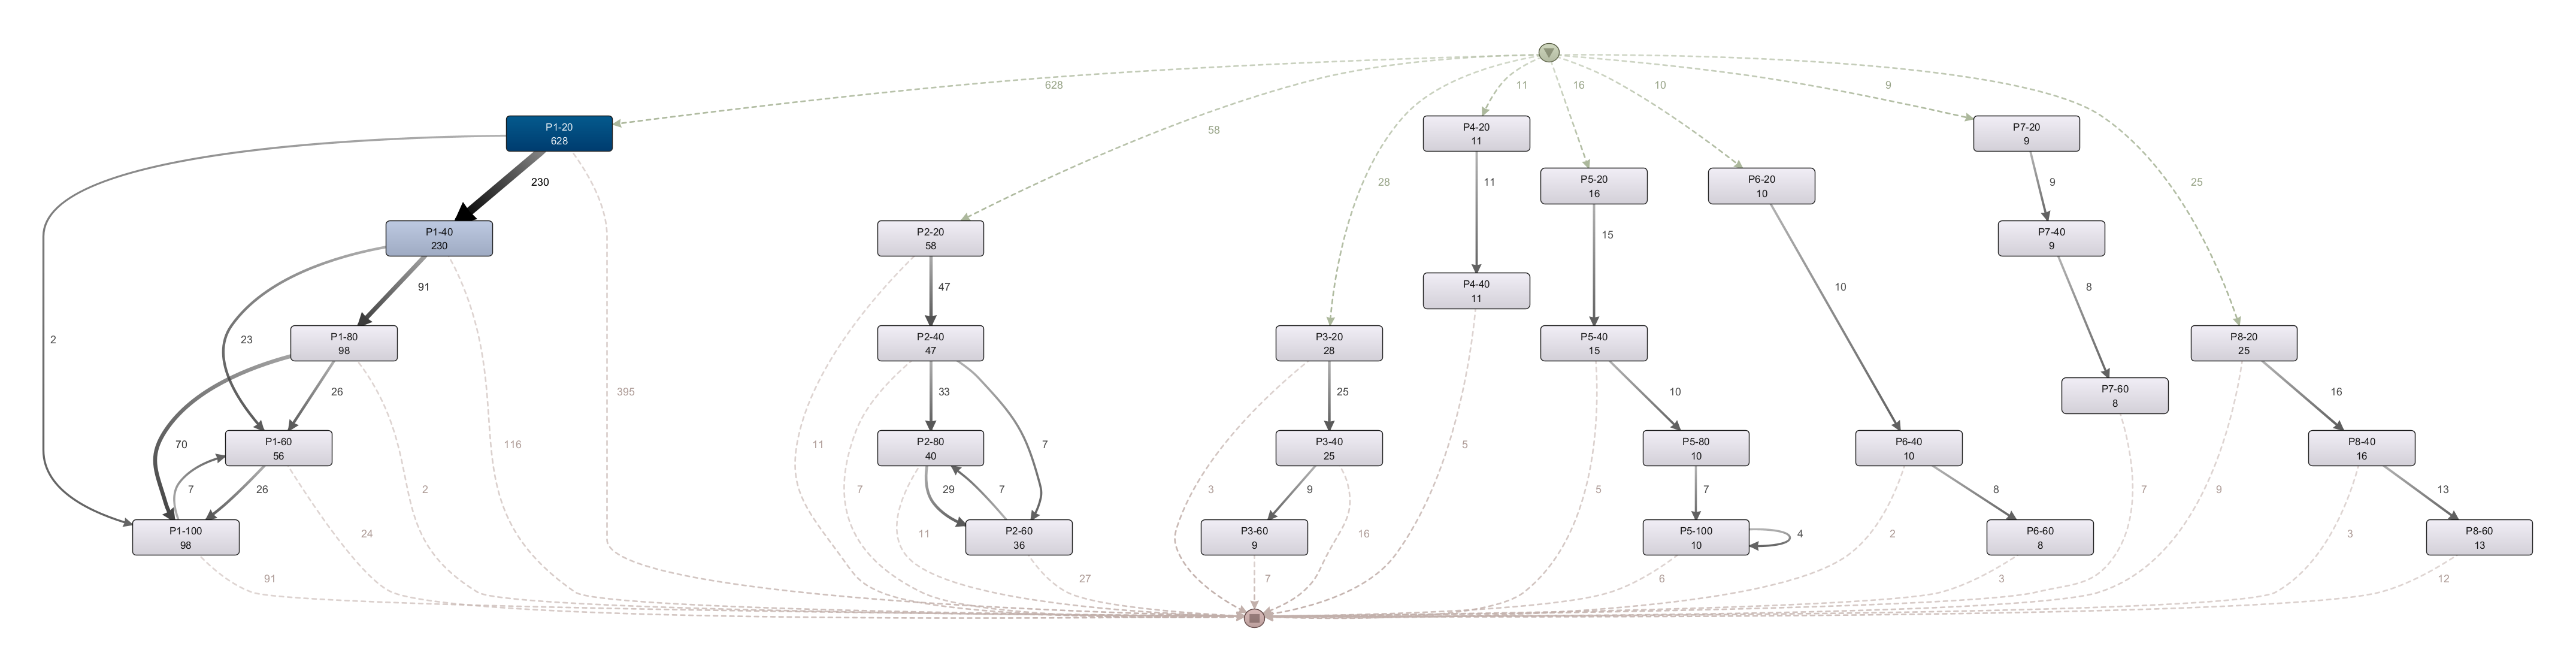
\includegraphics[width=\textwidth]{procesos/DBA1516P2GACompound.png}
    \caption{Análisis de procesos del grupo \texttt{DBA 1516 P2 GA} (\texttt{Activity} problema-milestone y \texttt{CaseId} sesión). Contiene el $60\%$ de las actividades y el $80\%$ de los caminos.}
    \label{fig:compoundDBA1516P2GA}
\end{figure}

Aunque Disco tiene mucho éxito y se pueden personalizar métricas e interpretaciones del conjunto de datos fuente, no se ajusta completamente a nuestros requerimientos para desvelar la estructura del comportamiento. Tras una larga experimentación con el programa Disco, se empiezan a ver sus limitaciones. En primer lugar, aunque Disco permite el filtrado de datos, si se quiere segmentar por grupos y extraer los procesos ocultos de cada uno de los grupos, hay que seleccionar el correspondiente grupo en el filtro, extraer los diagramas correspondientes e ir cambiándolo manualmente. Dado que tenemos un total de $77$ grupos de alumnos en los siete cursos académicos que forman parte del estudio (que pueden consultarse en las Tablas \ref{tab:groups1} y \ref{tab:groups2}), es inviable seguir usando el programa.

Así pues, en este trabajo fin de grado se ha implementado nuestra propia versión del programa, la herramienta de minería de procesos \emph{Graph Miner} en R, personalizada y adaptada a las necesidades del problema, basándose principalmente en la estructura principal de FuzzyMiner \cite{gunther2007fuzzy} con algunas adiciones menores.